\documentclass{article}

\usepackage{graphicx}
\usepackage{tikz}
\usepackage{tikzsymbols}
\usetikzlibrary{calc,patterns,shapes.geometric}
\pagestyle{empty}
\usepackage[margin=0pt]{geometry}
\geometry{papersize={14in,12in}}

\def\centerarc[#1](#2)(#3:#4:#5){\draw[#1] ($(#2)+({#5*cos(#3)},{#5*sin(#3)})$) arc (#3:#4:#5);}

\begin{document}
	\begin{figure}
		\centering
		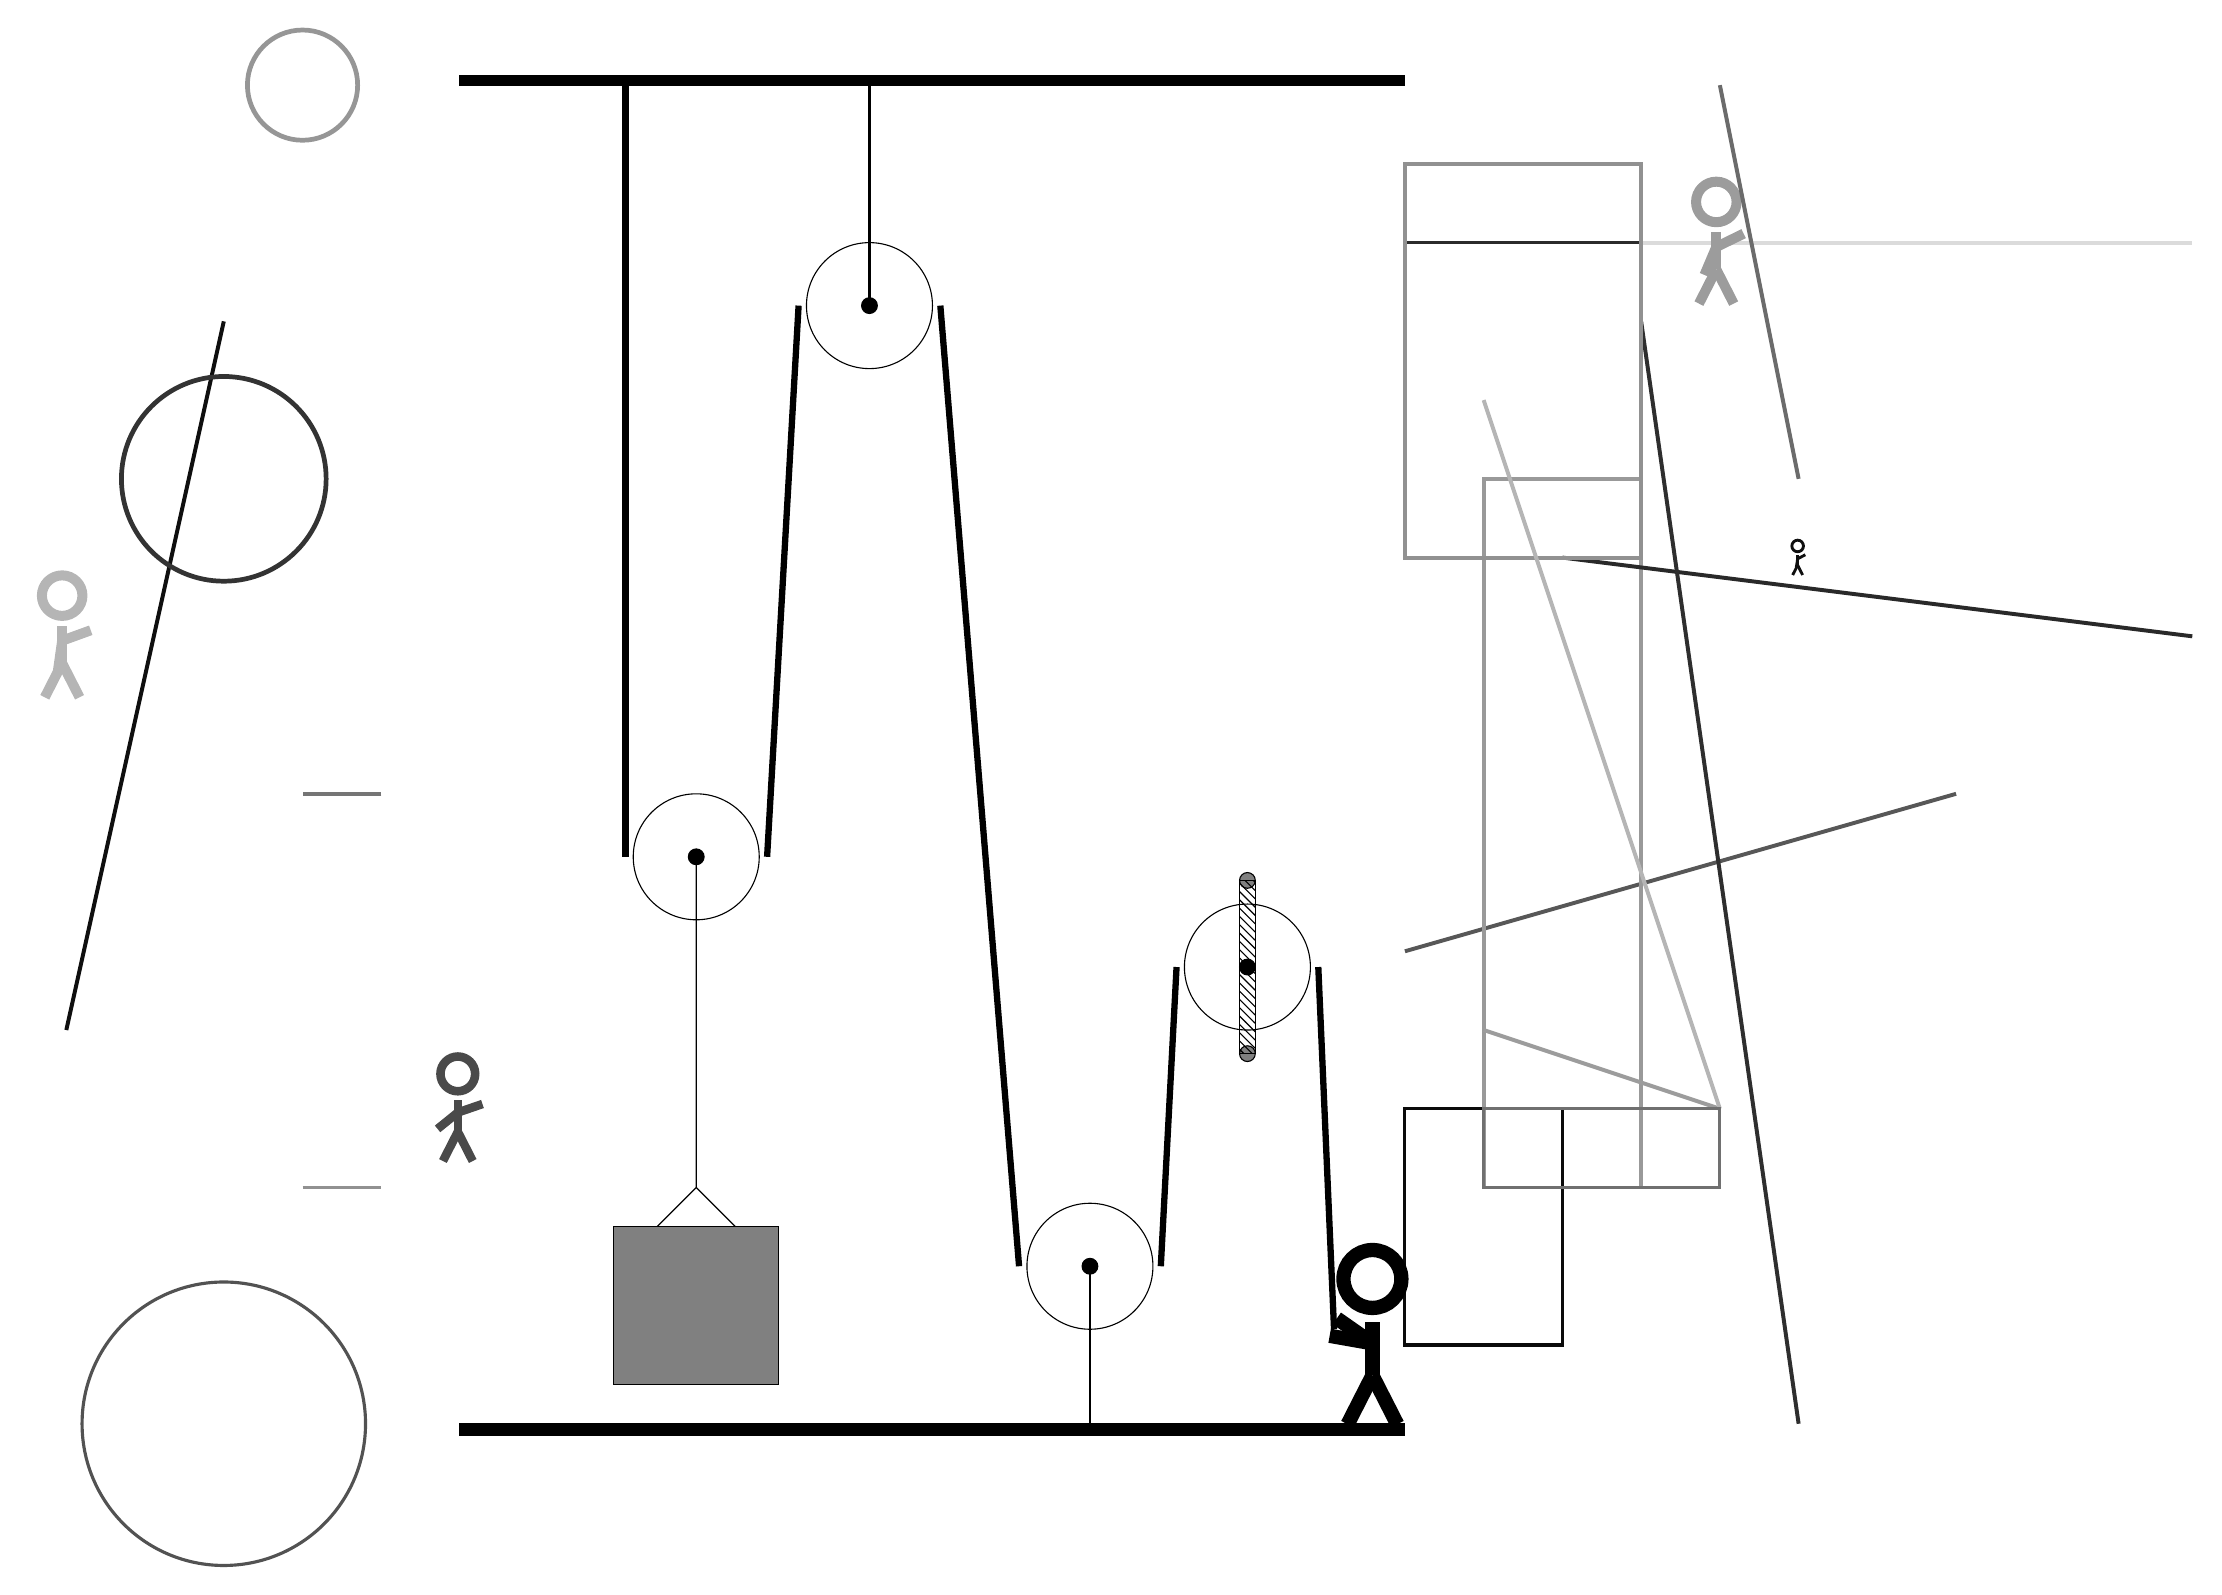
\begin{tikzpicture}
			%%%%% START %%%%%
			
			\draw[fill=black] (-2, 14) rectangle (10, 14.125);
			
			\draw (1, 4.2) circle (0.8);
			\draw[fill=black] (1, 4.2) circle (0.1);
			
			\draw (3.2, 11.2) circle (0.8);
			\draw[fill=black] (3.2, 11.2) circle (0.1);
			\draw[thick] (3.2, 11.2) -- (3.2, 14);
			
			\draw (6, -1) circle (0.8);
			\draw[fill=black] (6, -1) circle (0.1);
			\draw[thick] (6, -1) -- (6, -3);
			
			\draw[fill=white](8, 2.8) circle (0.8);
			\draw[fill=black] (8, 2.8) circle (0.1);
			\draw[fill=black!50] (8, 3.9) circle (0.1);
			\draw[fill=black!50] (8, 1.7) circle (0.1);
			\draw[pattern=north west lines, pattern color=black] (7.9, 3.9) rectangle (8.1, 1.7);
			
			\draw[line width=0.5mm, color=black!66](10, 3) -- (17, 5);
			
			\draw[line width=0.4mm, color=black!96] (10, -2) rectangle (12, 1);
			\draw[line width=0.5mm, color=black!94](-5, 11) -- (-7, 2);
			\draw[line width=0.5mm, color=black!14](13, 12) -- (20, 12);
			
			\draw[line width=0.5mm, color=black!40] (11, 0) rectangle (13, 9);
			\node[line width=0.6mm, color=black!39] at (14, 12) {\Strichmaxerl[7][67][26]};
			\draw[line width=0.4mm, color=black!83] (10, 8) rectangle (13, 12);
			\draw[line width=0.5mm, color=black!43](-4, 0) -- (-3, 0);
			\draw[line width=0.5mm, color=black!54](-3, 5) -- (-4, 5);
			
			\draw [line width=0.4mm, color=black!68](-5, -3) circle (1.8);
			\draw [line width=0.6mm, color=black!41](-4, 14) circle (0.7);
			\draw [line width=0.6mm, color=black!80](-5, 9) circle (1.3);
			\draw[line width=0.5mm, color=black!84](12, 8) -- (20, 7);
			
			\draw[line width=0.5mm, color=black!82](13, 11) -- (15, -3);
			\draw[line width=0.5mm, color=black!39](14, 1) -- (11, 2);
			\draw[line width=0.5mm, color=black!43] (10, 13) rectangle (13, 8);
			\node[line width=0.4mm, color=black!29] at (-7, 7) {\Strichmaxerl[7][82][20]};
			
			\draw[line width=0.5mm, color=black!29](14, 1) -- (11, 10);
			\node[line width=0.5mm, color=black!94] at (15, 8) {\Strichmaxerl[2][81][28]};
			
			\draw[line width=0.4mm, color=black!56] (11, 0) rectangle (14, 1);
			\draw[line width=0.5mm, color=black!58](14, 14) -- (15, 9);
			
			\node[line width=0.5mm, color=black!71] at (-2, 1) {\Strichmaxerl[6][39][19]};
			
			
			\draw (1, 4.2) -- (1, 0) -- (0.5, -0.5);
			\draw (1, 0) -- (1.5, -0.5);
			\draw[fill=black!50] (-0.05, -0.5) rectangle (2.05, -2.5);
			
			\draw[line width=0.8mm] (0.1, 14) -- (0.1, 4.2);
			\centerarc[line width=0.8mm](1, 4.2)(180:360:0.9);
			\draw[line width=0.8mm](1.9, 4.2) -- (2.3, 11.2);
			\centerarc[line width=0.8mm](3.2, 11.2)(0:180:0.9);
			\draw[line width=0.8mm](4.1, 11.2) -- (5.1, -1);
			\centerarc[line width=0.8mm](6, -1)(180:360:0.9);
			\draw[line width=0.8mm](6.9, -1) -- (7.1, 2.8);
			\centerarc[line width=0.8mm](8, 2.8)(0:180:0.9);
			\draw[line width=0.8mm](8.9, 2.8) -- (9.1, -1.8);
			
			\node at (9.5, -1.9) {\Strichmaxerl[10][-35][170]};
			
			\draw[fill=black] (-2, -3) rectangle (10, -3.15);
			
			%%%%% END %%%%%
		\end{tikzpicture}
	\end{figure}	
\end{document}